\section{Research}


\subsection{June 17-20 \texorpdfstring{$\mu(C_\mathcal{B}^2(Q, V, \alpha)) = 0 \Rightarrow \mu(C_\mathcal{B}(x, V, \alpha)) = 0$}{Lg}}
\begin{lemma}\label{lemmaCQ1=CQ2}
    Let $x\in H, \alpha\in(0,1)$ and $V$ be an $m$-dimensional linear plane. If for every dyadic cube $Q\ni x$ with side length $2^{-k}, k\in\mathbb{N}$
    \begin{equation}\label{muB2=0}
        \mu(C_\mathcal{B}^2(Q, V, \alpha)) = 0
    \end{equation}
    then
    \begin{equation}\label{muBx=0}
        \mu(C_\mathcal{B}(x, V, \alpha)) = 0
    \end{equation}
\end{lemma}
\textit{Proof}. Let $Q_{k}$ denote a dyadic cube with side length $2^{-k}, k\in\mathbb{N}$ in the fixed cube system. Then for any two different points in $Q_k$, we have $0<|x_1-x_2|\leq \sqrt{C}\cdot 2^{-k}, \forall x_1, x_2\in Q_k$ where $C$ is the constant and particularly $C=n$ when in $\rr^n$. When $k\rightarrow \infty, 2^{-k}\rightarrow 0$ so there exists $N\in\nn$ such that whenever $k\geq N$, we have $|x_1-x_2|<\alpha\epsilon/2<\epsilon/2, \forall \epsilon >0$ for choosing $x_1, x_2$ still in the $Q_k\ni x$. Now consider that if $y\in C_\mathcal{B}(x_1, V, \alpha)$, we have $\dist(y-x_1, V) > \alpha|y-x_1|$ by definition of bad cones. Choose
$$\epsilon\leq \frac{\dist(y-x_1, V)-\alpha|y-x_1|}{\alpha}\Rightarrow \dist(y-x_1, V) \geq \alpha (|y-x_1|+\epsilon),$$
so that
\begin{equation*}
    \begin{aligned} 
        \dist\left(y-x_{2}, V\right) & \geq \dist(y-x_1, V)-\left|x_1-x_2\right| \\ 
        & \geq \alpha(|y-x_1|+\epsilon)-\alpha(\epsilon / 2) \\ 
        & =\alpha(|y-x_1|+\epsilon / 2) \\ 
        & >\alpha\left(|y-x_1|+\left|x_2-x_1\right|\right) \\ 
        & \geq \alpha\left(\left|y-x_2\right|\right) 
\end{aligned}
\end{equation*}
It follows that $y\in C_{\mathcal{B}}(x_2, V, \alpha)$, so $ C_{\mathcal{B}}(x_1, V, \alpha)\subseteq C_{\mathcal{B}}(x_2, V, \alpha)$. If we exchange $x_1$ and $x_2$ for the proof, it is also true that $ C_{\mathcal{B}}(x_2, V, \alpha)\subseteq C_{\mathcal{B}}(x_1, V, \alpha)$. Thus, $ C_{\mathcal{B}}(x_1, V, \alpha)=C_{\mathcal{B}}(x_2, V, \alpha)$. Since $x_1, x_2$ are arbitrary points in $Q_k$, we have 
\begin{equation}\label{CB2=CB1}
    \lim_{k\rightarrow \infty} C_\mathcal{B}^2(Q_k, V, \alpha) = \lim_{k\rightarrow \infty} \bigcap_{x\in Q_k} C_\mathcal{B}(x, V, \alpha) = \lim_{k\rightarrow \infty} \bigcup_{x\in Q_k}C_\mathcal{B}(x, V, \alpha) = \lim_{k\rightarrow\infty}C_\mathcal{B}^1(Q_k, V, \alpha)
\end{equation}
For any $Q\ni x$, we can do this process for any $Q_k\in Q, Q_k\ni x$, so applyin (\ref{CB2=CB1}) and (\ref{muB2=0}), for each $Q\ni x$,
\begin{equation*}
    \begin{aligned}
        \mu(\bigcup_{x\in Q}C_\mathcal{B}(x, V, \alpha))
        &= \mu(C_\mathcal{B}^1(Q, V, \alpha)) \\
        &= \lim_{k\rightarrow\infty}\mu(\bigcup_{Q_k\in Q} C_\mathcal{B}^1(Q_k, V, \alpha))\\
        &= \lim_{k\rightarrow\infty}\mu(\bigcup_{Q_k\in Q} C_\mathcal{B}^2(Q_k, V, \alpha))\\
        &= 0
    \end{aligned}
\end{equation*}
Therefore, by doing the same process for all $Q\ni x$, we have (\ref{muBx=0}). \\
An example of this proof illustrated in $\rr^2$ is shwon in Figure \ref{fig:CB1=CB2}.

\begin{figure}[H]
    \centering
    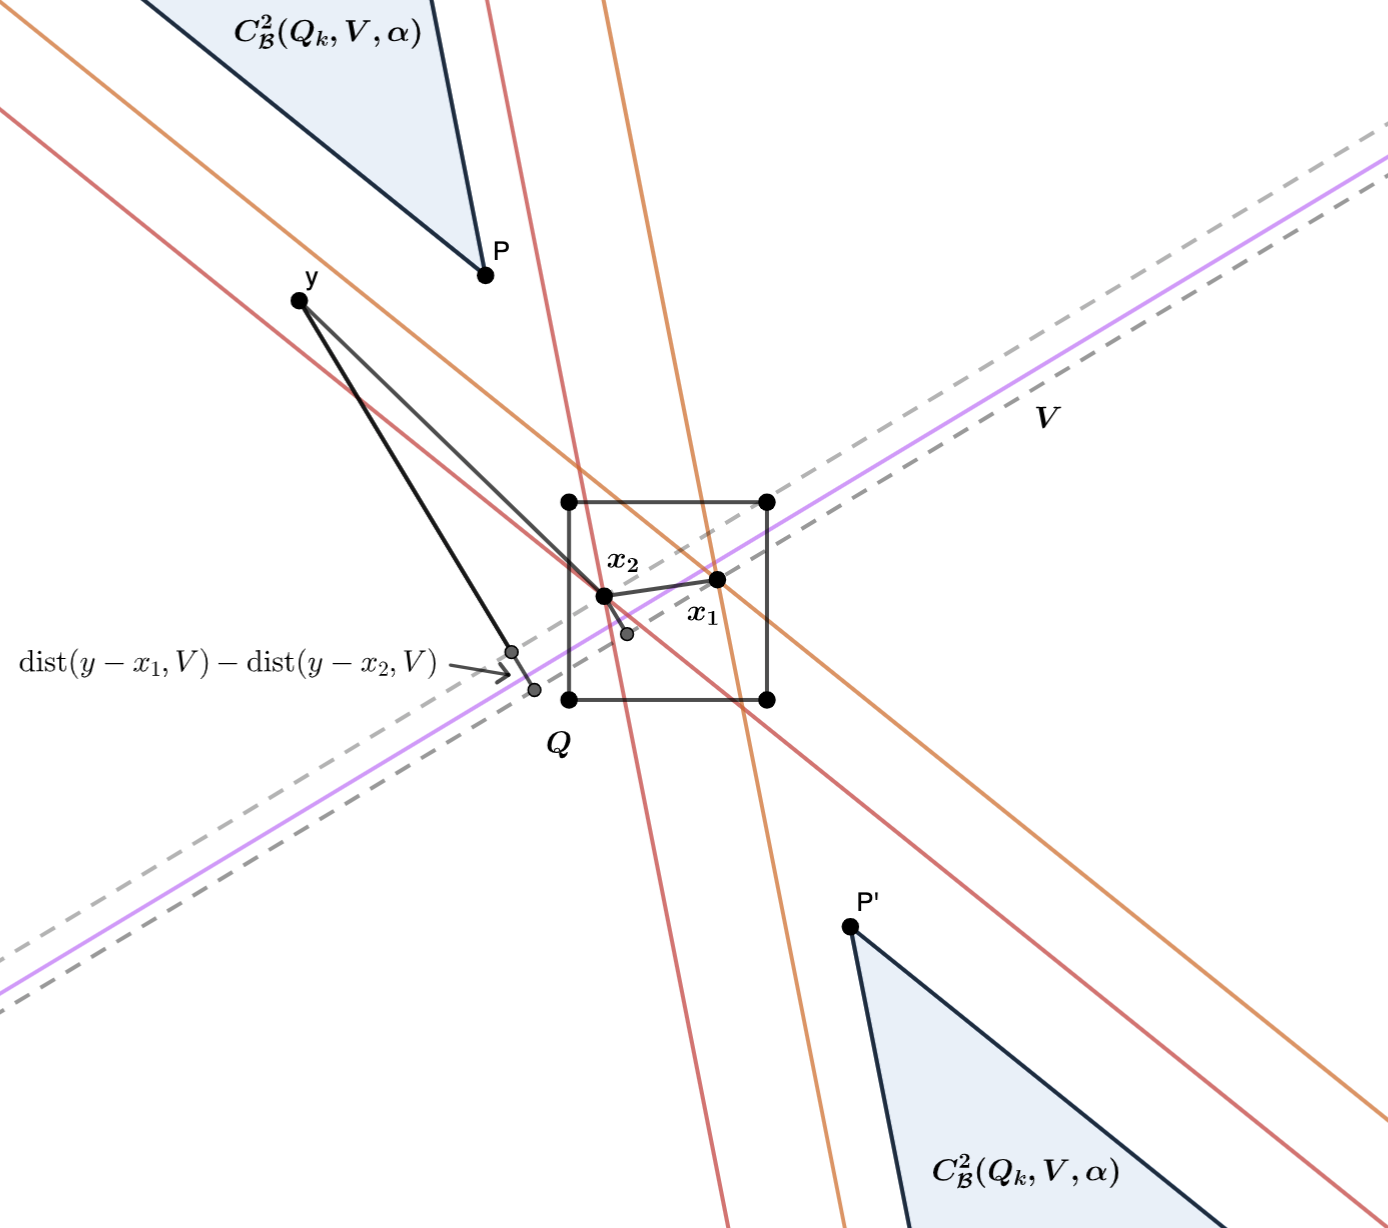
\includegraphics[width=.6\textwidth]{images/CB1=CB2.png}
    \caption{Example visulization of proof in $\rr^2$}
    \label{fig:CB1=CB2}
\end{figure}


\begin{corollary}[{\cite[Corollary 7.1]{naples2020}}]\label{LisaCoro7.1}
    Let $\mu$ be a Radon measure on $H, V$ be an $m$-dimensional linear plane in $H$, $\alpha \in(0,1)$, and $0<r<\infty$. If for $\mu$ -a.e. $x \in H$
   $$
   \mu\left(C_{\mathcal{B}}(x, r, V, \alpha)\right)=0
   $$
   then $\mu$ is carried by $m$-Lipschitz graphs.
\end{corollary}

   

\begin{corollary}
    Suppose that at $\mu$-a.e. $x$, $\alpha\in(0, 1)$, for all $k$, for every cube $Q\ni x$ of side length $2^{-k}, k\in\nn$ satisfies
    $$
    \mu(C^2_\mathcal{B}(Q, V, \alpha)) = 0
    $$ 
    then $\mu$ is carried by $m$-Lipschitz graphs
\end{corollary}
\begin{proof}
    Applying Lemma \ref{lemmaCQ1=CQ2}, we have $\mu(C_\calB(x, V, \alpha)) = 0$ and applying corollary \ref{LisaCoro7.1}, we obtain the desired conclusion. 
\end{proof}


\newpage
\subsection{June 16 New Cone Definition for Dyadic Cubes}
\begin{definition}[Dyadic Cubes]
    $$
Q=\left[\frac{j_{1}}{2^{k}}, \frac{j_{1}+1}{2^{k}}\right) \times \cdots \times\left[\frac{j_{n}}{2^{k}}, \frac{j_{n}+1}{2^{k}}\right), \quad k, j_{1}, \ldots, j_{n} \in \mathbb{Z}
$$
\end{definition}

\begin{definition}[Bad Cone at a Cube(definition 1)] Let $Q$ be the dyadic cube, then we can have the first definition of bad cone at $Q$ with respect to $V$ and $\alpha$ by:
    $$C^1_{\mathcal{B}}(Q, V, \alpha) := \bigcup_{x\in Q} C_\mathcal{B}(x, V, \alpha), \quad C^1_{\mathcal{B}}(Q, r, V, \alpha) = C^1_{\mathcal{B}}(Q, V, \alpha) \cap B(x,r)$$
    where $V$ is a m-dimensional linear plane through the origin. 
\end{definition}

\begin{definition}[Bad Cone for Cube(definition 2)]
    We can have the second definition of bad cone at $Q$ with respect to $V$ and $\alpha$ with the similar notation:
    $$C^2_{\mathcal{B}}(Q, V, \alpha) := \bigcap_{x\in Q} C_\mathcal{B}(x, V, \alpha), \quad
    C^2_{\mathcal{B}}(Q, r, V, \alpha) = C^2_{\mathcal{B}}(Q, V, \alpha) \cap B(x,r)
    $$
\end{definition}
\begin{figure}[H]
    \centering
    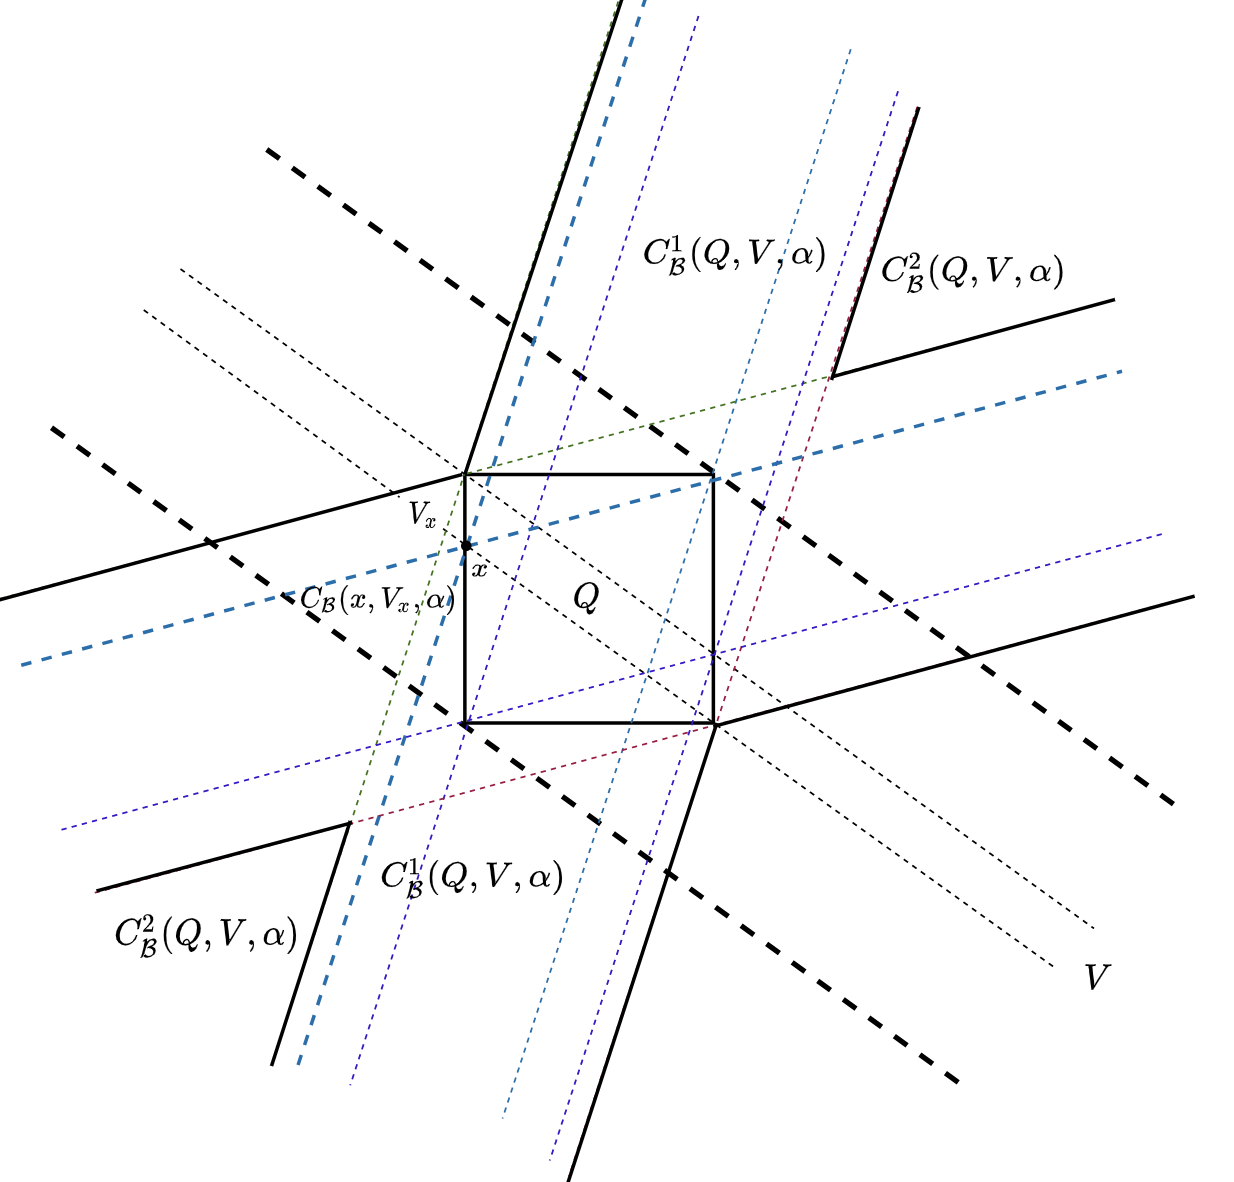
\includegraphics[width=.66\textwidth]{images/cubebadconeDef.png}
    \caption{Visulize two definitions of bad cone at a cube in $\rr^2$}
\end{figure}

\begin{problem}
    Suppose that at $\mu$-a.e. $x$, $\alpha\in(0, 1)$, for all $k$, for every cube $Q\ni x$ of side length $2^{-k}$ satisfies
    $$
    \mu(C^2_\mathcal{B}(Q, V, \alpha)) = 0
    $$ 
    is $\mu$-carried Lipschitz by Lipschitz graphs?
\end{problem}

\newpage
\subsection{June 15 A Proposition of Doubling Measure for Cubes}

\begin{proposition}
    If $\forall x\in \rr^2, \mu(B(x, 2r))\leq K\mu(B(x,r)), K\in\zz^+$, then $\exists R\in \zz^+$ s.t. $\mu(3Q)\leq R\mu(Q)$ where $Q$ is the cube, 3$Q$ is the cube with triple side length with same center as $Q$. 
\end{proposition}
\proof  $\mu(3Q) \leq \mu(B(x, 4r)) \leq K^2\mu(B(x, r))\leq K^2 \mu(Q)$ due to doubling measure and containment. 

\begin{figure}[H]
    \centering
    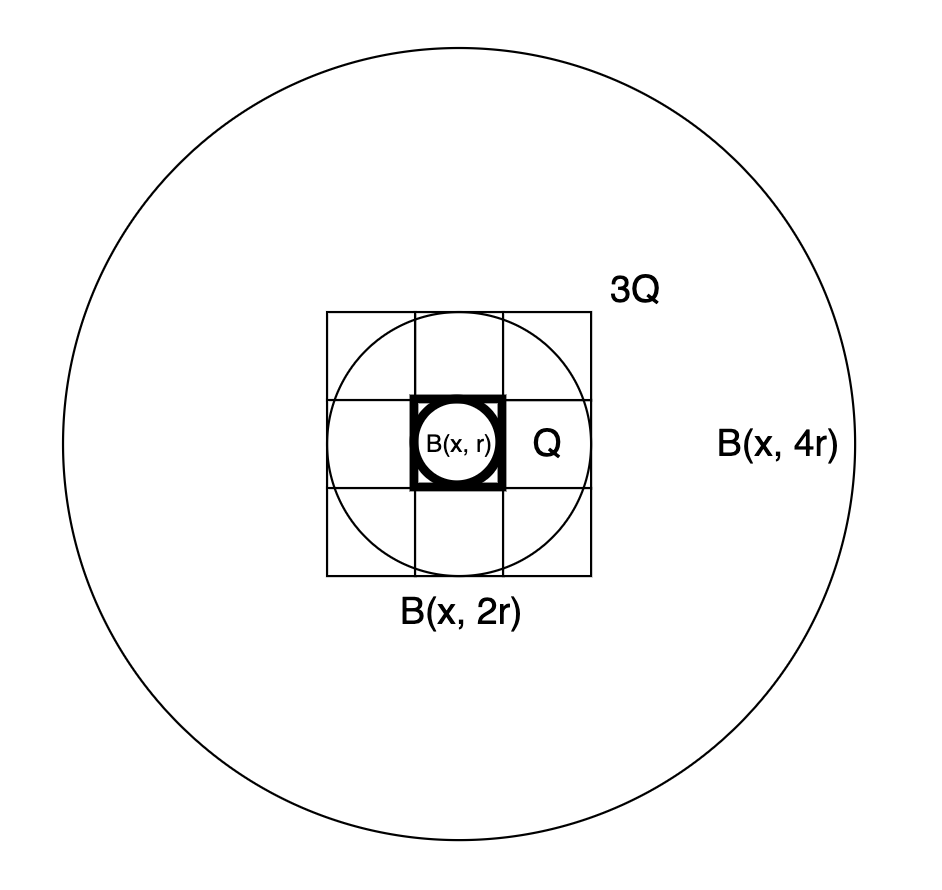
\includegraphics[width=.66\textwidth]{images/doubleMcube.png}
\end{figure}


\newpage
\subsection{June 14 Paper \texorpdfstring{\cite{naples2020}}{Lg} Sec. 7 Graph Rectifiable Measures}

\begin{definition}[Good Cone]
    Let $V$ be a m-dimensional plane in Hilbert space $H$, then we can define the good cone at $x$ with respect to $V$ and $\alpha$ by:
    $$
    C_\mathcal{G}(x, V, \alpha) := \{y\in H: \dist(y-x, V) \leq \alpha |x-y|\}
    $$
    another notation:
    $$
    C_\mathcal{G}(x, r, V, \alpha) = C_\mathcal{G}(x, V, \alpha) \cap B(x, r)
    $$
\end{definition}
\begin{definition}[Bad Cone]
    The bad cone at x with respect to V and $\alpha$:
    $$
    C_\mathcal{B}(x, V, \alpha) := H\setminus C_{\mathcal{G}(x, V, \alpha)}, \quad C_\mathcal{B}(x, r, V, \alpha) = C_\mathcal{B}(x, V, \alpha) \cap B(x, r)
    $$
\end{definition}


\begin{figure}[H]
    \centering
    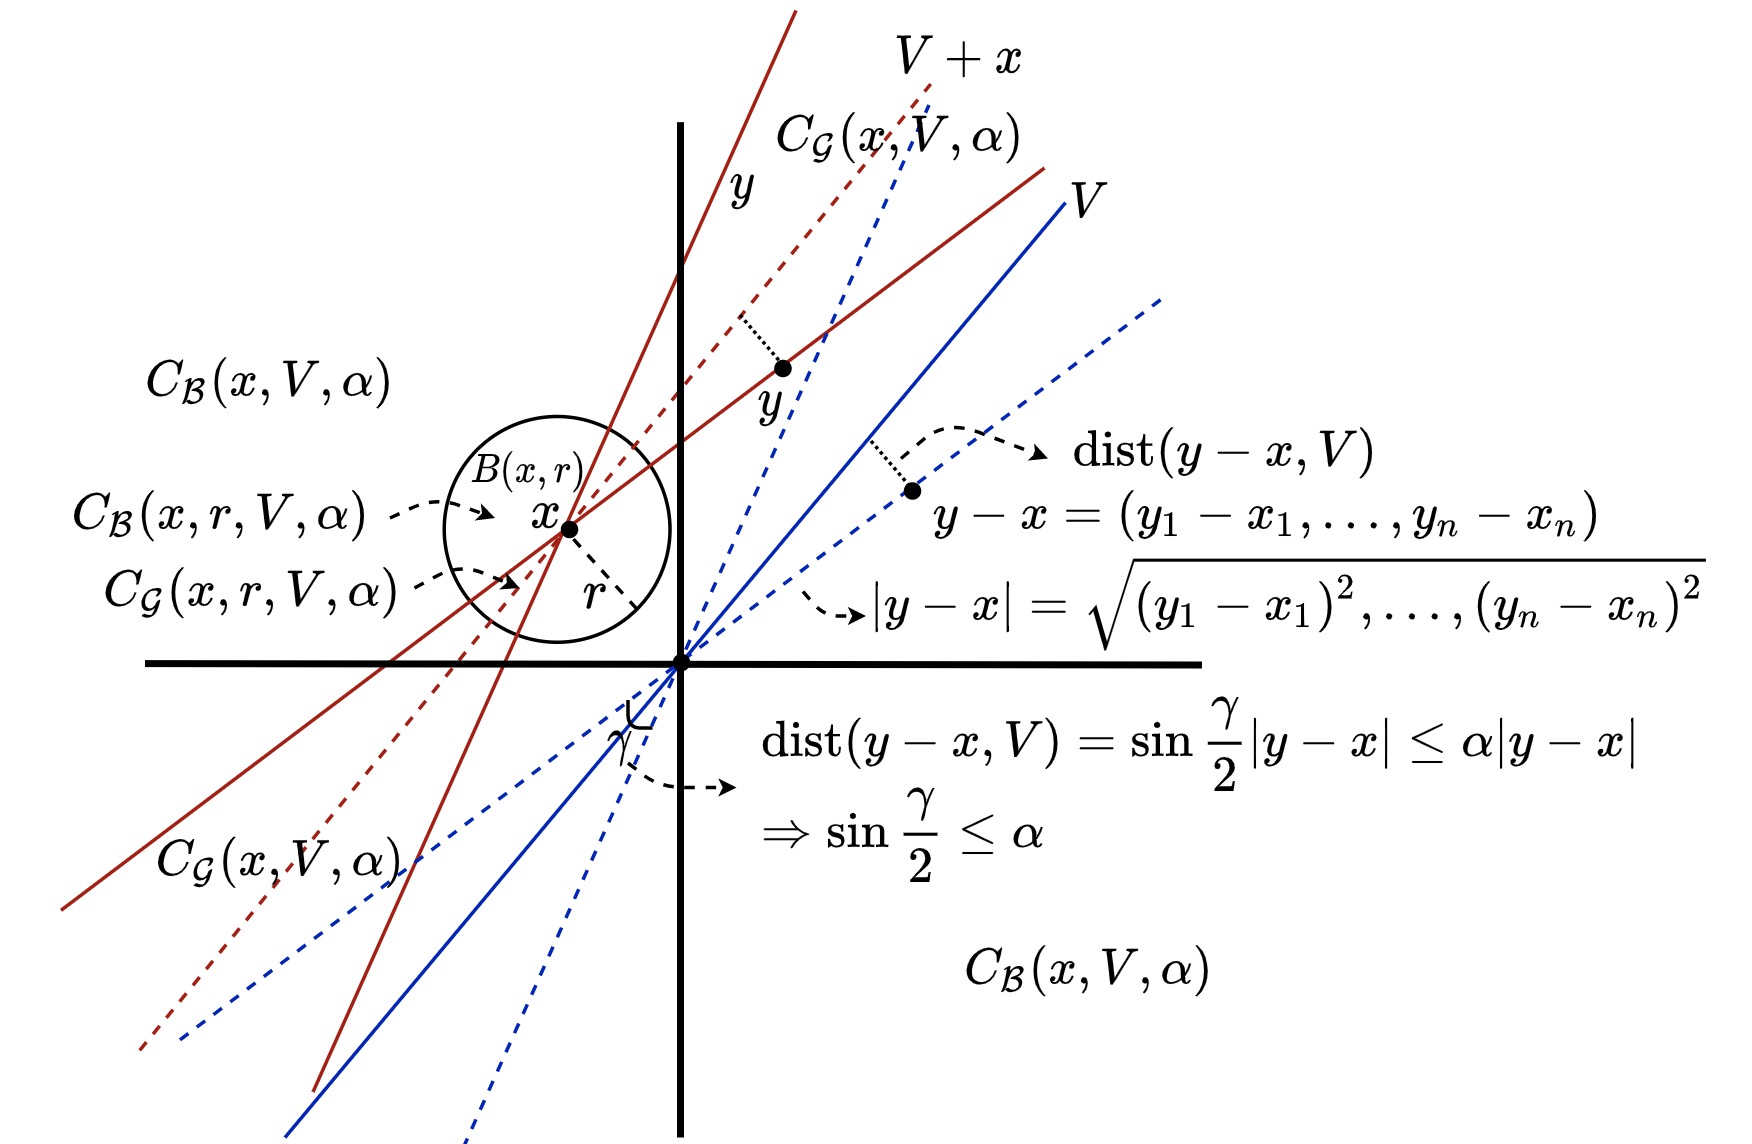
\includegraphics[width=.8\textwidth]{images/conedef.png}
    \caption{Example visualization of definitions related to cones in $\rr^2$}
\end{figure}

\begin{definition}[Carried $\&$ Singular]
   Let $(\mathbb{X}, \mathcal{M})$ be a measurable space, and let $\mathcal{N} \subset \mathcal{M}$ be a family of measurable sets. We say
   \begin{enumerate}[(1)]
       \item $\mu$ is carried by $\mathcal{N}$ if there exist countably many $N_{i} \in \mathcal{N}$ such that $\mu\left(\mathbb{X} \backslash \bigcup_{i} N_{i}\right)=0$;
       \item $\mu$ is singular to $\mathcal{N}$ if $\mu(N)=0$ for every $N \in \mathcal{N}$.    
   \end{enumerate}
   A $\sigma$ -finite measure $\mu$ on $(\mathbb{X}, \mathcal{M})$ can be decomposed uniquely as
       $$
       \mu=\mu_{\mathcal{N}}+\mu_{\mathcal{N}}^{\perp}
       $$
       where $\mu_{\mathcal{N}}$ is carried by $\mathcal{N}$ and $\mu_{\mathcal{N}}^{\perp}$ is singular to $\mathcal{N}$. 
\end{definition}

\begin{theorem}[Theorem 7.1 Geometric Lemma] $ $\\
    Let $F \subset H$, let $V$ be an $m$-dimensional linear plane in $H$, and let $\alpha \in(0,1) .$ If
$$
F \backslash C_{\mathcal{G}}(x, V, \alpha)=\emptyset \text { for all } x \in F
$$
then $F$ is contained in an $m$ -Lipschitz graphs. In particular, $F \subset \Gamma$ where $\Gamma$ is a Lipschitz graph with respect to $V$ and the Lipschitz constant corresponding to $\Gamma$ is at most $1+1 /\left(1-\alpha^{2}\right)^{1 / 2} .$
\end{theorem}
\proof Let $x \in F$. Let $P_{V}: H \rightarrow V$ denote standard projection onto the $m$ -plane $V$. Suppose that $\left|P_{V} x-P_{V} y\right|<\left(1-\alpha^{2}\right)^{1 / 2}|x-y|$. Then $y \in C_{\mathcal{B}}(x, V, \alpha)$, and by assumption of $F$ this means that $y \notin F$. Thus we may assume that if $x, y \in F$ then
$$
\left|P_{V} x-P_{V} y\right| \geq\left(1-\alpha^{2}\right)^{1 / 2}|x-y|
$$
From this inequality we see that $P_{V} \mid F$ is one-to-one with Lipschitz inverse $f=\left(P_{V} \mid F\right)^{-1}$ and $\operatorname{Lip}(f) \leq\left(1-\alpha^{2}\right)^{-1 / 2}$. Note that $F=f\left(P_{V} \mid F\right)$. Then there exists a Lipschitz extension $\tilde{f}: V \rightarrow$ $H$ so that $F \subset \tilde{f}(V)$. Thus the desired result holds. 

\begin{corollary}[Corollary 7.1]
 Let $\mu$ be a Radon measure on $H, V$ be an $m$-dimensional linear plane in $H$, $\alpha \in(0,1)$, and $0<r<\infty$. If for $\mu$ -a.e. $x \in H$
$$
\mu\left(C_{\mathcal{B}}(x, r, V, \alpha)\right)=0
$$
then $\mu$ is carried by $m$ -Lipschitz graphs.
\end{corollary}
\proof Let $F$ denote the set of $x \in H$ that satisfy (18). We may assume $F \subset B(0, r / 2)$; otherwise we may write $F$ as a union of countably many sufficiently small sets and show that each one is $m$ -graph rectifiable. Let $\left\{x_{i}\right\}$ be a countable dense subset of $F .$ It follows from (18) and the containment $F \subset B(0, r / 2)$ that for each $x_{i}$ there exists $F_{i} \subset F$ such that
$$
F_{i} \cap C_{\mathcal{B}}\left(x_{i}, r, V, \alpha\right)=F_{i} \cap C_{\mathcal{B}}\left(x_{i}, V, \alpha\right)=\emptyset
$$
and $\mu\left(F \backslash F_{i}\right)=0$. Define $F^{\prime}:=\bigcap_{i=1}^{\infty} F_{i}$. Then
$$
\mu\left(F \backslash F^{\prime}\right)=\mu\left(F \backslash \bigcap_{i=1}^{\infty} F_{i}\right)=\mu\left(\bigcup_{i=1}^{\infty} F \backslash F_{i}\right) \leq \sum_{i=1}^{\infty} \mu\left(F \backslash F_{i}\right)=0
$$
We claim that $F^{\prime} \cap C_{\mathcal{B}}(x, V, \alpha)=\emptyset$ for every $x \in F^{\prime} .$ Fix $x \in F^{\prime}$, and let $y \in C_{\mathcal{B}}(x, V, \alpha)$.
By definition of bad cone we have that $\dist(y-x, V)>\alpha|y-x|$. Now let $\epsilon>0$ such that $\dist(y-x, V) \geq \alpha(|y-x|+\epsilon)$. Recalling that $0<\alpha<1$, choose $x_{i}$ such that $\left|x_{i}-x\right|<\alpha \epsilon / 2<$
$\epsilon / 2 .$ Then
$$
\begin{aligned}
\dist\left(y-x_{i}, V\right) & \geq \dist(y-x, V)-\left|x-x_{i}\right| \\
& \geq \alpha(|y-x|+\epsilon)-\alpha(\epsilon / 2) \\
&=\alpha(|y-x|+\epsilon / 2) \\
&>\alpha\left(|y-x|+\left|x_{i}-x\right|\right) \\
& \geq \alpha\left(\left|y-x_{i}\right|\right) .
\end{aligned}
$$
In particular, we conclude that $y \in C_{\mathcal{B}}\left(x_{i}, V, \alpha\right) .$ Since $F_{i} \cap C_{\mathcal{B}}\left(x_{i}, V, \alpha\right)=\emptyset$, it must be that case that $y \notin F_{i}$. It follows that $y \notin F^{\prime}$, and thus $F^{\prime} \cap C_{\mathcal{B}}(x, V, \alpha)=\emptyset$ for all $x \in F^{\prime}$. By an application of Theorem $7.1$ we conclude that there exists an $m$ -Lipschitz graph $\Gamma$ such that $F^{\prime} \subset \Gamma$, so $\mu(F \backslash \Gamma)=0$.

\begin{lemma}[Lemma 7.2]
    Let $\mu$ be a Radon measure on $H$. For $x_{0} \in H, V$ an $m$-dimensional linear plane, $\alpha \in(0,1)$, and parameter $K>0$, let $E$ denote the set of points $x \in H$ such that
(i) The sequence of functions
$$
f_{r}(x):=\frac{\mu\left(C_{\mathcal{B}}(x, r, V, \alpha)\right)}{\mu(B(x, r))}
$$
converges to 0 uniformly on $E$, and
(ii) there exists $r_{1}>0$ such that at every $x \in E$,
$$
\mu(B(x, 2 r)) \leq K \mu(B(x, r)) \text { for all } r \in\left(0, r_{1}\right]
$$
Then $E$ is $\mu$ -carried by $m$ -Lipschitz graphs with Lipschitz constants depending on at most $K$ and $\alpha .$
\end{lemma}
\proof Fix $\delta>0$. By uniform convergence, choose $r_{\delta} \leq r_{1}$ such that for all $r<r_{\delta}$ and for all $x \in E$
(19)
$$
\frac{\mu\left(C_{\mathcal{B}}(x, 2 r, V, \alpha)\right)}{\mu(B(x, 2 r))}<\delta
$$
Fix $x \in E$, and define $S:=E \cap C_{\mathcal{B}}(x, r, V, 2 \alpha)$. Assuming the set is non-empty, fix $y_{0} \in S$ such that $\left|x-y_{0}\right|=\max _{y \in S}|a-y|=: \lambda r$ for some $0<\lambda \leq 1$. As an application of Lemma $7.1$ choose $\eta_{\alpha}$ such that $B\left(y_{0}, \eta_{\alpha} \lambda r\right) \subset C_{\mathcal{B}}(x, 2 r, V, \alpha) .$ Let $d=\log _{2}\left(\frac{\lambda+2}{\eta_{\alpha} \lambda}\right)$. Then
$$
2^{d} \eta_{\alpha} \lambda r=\frac{\lambda+2}{\eta_{\alpha} \lambda} \eta_{\alpha} \lambda r=(\lambda+2) r=\left|x-y_{0}\right| r+2 r .
$$
In particular, for the specified value of $d, B(x, 2 r) \subset B\left(y_{0}, 2^{d} \eta_{\alpha} \lambda r\right) .$ Applying condition (ii) of the set $E$ at the point $y_{0}$ we see that
$(20)$
$\mu\left(C_{\mathcal{B}}(x, 2 r, V, \alpha)\right) \geq \mu\left(B\left(x, \eta_{\alpha} \lambda r\right)\right) \geq K^{-d} \mu\left(B\left(y_{0}, 2^{d} \eta_{\alpha} \lambda r\right)\right) \geq K^{-d} \mu(B(x, 2 r))$
Combining inequalities (19) and (20), we get the density ratio bounds
$$
\delta>\frac{\mu\left(C_{\mathcal{B}}(x, 2 r, V, \alpha)\right)}{\mu(B(x, 2 r))} \geq K^{-d}
$$
for all $r<r_{\delta}$. In particular, this implies that $d>\frac{-\log (\delta)}{\log K}$. Equivalently,
$$
\log \left(\frac{\lambda+2}{\eta_{\alpha} \lambda}\right)>\frac{-\log \delta}{\log K}
$$
so that if $\delta$ is chosen to be less than $2^{-\log K \log \left(\frac{5}{\eta_{\alpha}}\right)}$ then $\lambda<\frac{1}{2}$. From this result we conclude that for $r<r_{\delta}$ and for all $y \in S,|x-y|<\frac{1}{2} r$. Letting $r \downarrow 0$ we conclude that $\mu\left(E \cap C_{\mathcal{B}}\left(x, r_{\delta}, V, 2 \alpha\right)\right)=0$. Thus we can apply Corollary $7.1$, and we obtain the desired conclusion. 

